\PassOptionsToPackage{unicode=true}{hyperref} % options for packages loaded elsewhere
\PassOptionsToPackage{hyphens}{url}
%
\documentclass[ignorenonframetext,]{beamer}
\usepackage{pgfpages}
\setbeamertemplate{caption}[numbered]
\setbeamertemplate{caption label separator}{: }
\setbeamercolor{caption name}{fg=normal text.fg}
\beamertemplatenavigationsymbolsempty
% Prevent slide breaks in the middle of a paragraph:
\widowpenalties 1 10000
\raggedbottom
\setbeamertemplate{part page}{
\centering
\begin{beamercolorbox}[sep=16pt,center]{part title}
  \usebeamerfont{part title}\insertpart\par
\end{beamercolorbox}
}
\setbeamertemplate{section page}{
\centering
\begin{beamercolorbox}[sep=12pt,center]{part title}
  \usebeamerfont{section title}\insertsection\par
\end{beamercolorbox}
}
\setbeamertemplate{subsection page}{
\centering
\begin{beamercolorbox}[sep=8pt,center]{part title}
  \usebeamerfont{subsection title}\insertsubsection\par
\end{beamercolorbox}
}
\AtBeginPart{
  \frame{\partpage}
}
\AtBeginSection{
  \ifbibliography
  \else
    \frame{\sectionpage}
  \fi
}
\AtBeginSubsection{
  \frame{\subsectionpage}
}
\usepackage{lmodern}
\usepackage{amssymb,amsmath}
\usepackage{ifxetex,ifluatex}
\usepackage{fixltx2e} % provides \textsubscript
\ifnum 0\ifxetex 1\fi\ifluatex 1\fi=0 % if pdftex
  \usepackage[T1]{fontenc}
  \usepackage[utf8]{inputenc}
  \usepackage{textcomp} % provides euro and other symbols
\else % if luatex or xelatex
  \usepackage{unicode-math}
  \defaultfontfeatures{Ligatures=TeX,Scale=MatchLowercase}
\fi
\usetheme[]{AnnArbor}
\usecolortheme{dove}
% use upquote if available, for straight quotes in verbatim environments
\IfFileExists{upquote.sty}{\usepackage{upquote}}{}
% use microtype if available
\IfFileExists{microtype.sty}{%
\usepackage[]{microtype}
\UseMicrotypeSet[protrusion]{basicmath} % disable protrusion for tt fonts
}{}
\IfFileExists{parskip.sty}{%
\usepackage{parskip}
}{% else
\setlength{\parindent}{0pt}
\setlength{\parskip}{6pt plus 2pt minus 1pt}
}
\usepackage{hyperref}
\hypersetup{
            pdftitle={STAD29: Statistics for the Life and Social Sciences},
            pdfauthor={Lecture notes},
            pdfborder={0 0 0},
            breaklinks=true}
\urlstyle{same}  % don't use monospace font for urls
\newif\ifbibliography
\usepackage{color}
\usepackage{fancyvrb}
\newcommand{\VerbBar}{|}
\newcommand{\VERB}{\Verb[commandchars=\\\{\}]}
\DefineVerbatimEnvironment{Highlighting}{Verbatim}{commandchars=\\\{\}}
% Add ',fontsize=\small' for more characters per line
\usepackage{framed}
\definecolor{shadecolor}{RGB}{248,248,248}
\newenvironment{Shaded}{\begin{snugshade}}{\end{snugshade}}
\newcommand{\AlertTok}[1]{\textcolor[rgb]{0.94,0.16,0.16}{#1}}
\newcommand{\AnnotationTok}[1]{\textcolor[rgb]{0.56,0.35,0.01}{\textbf{\textit{#1}}}}
\newcommand{\AttributeTok}[1]{\textcolor[rgb]{0.77,0.63,0.00}{#1}}
\newcommand{\BaseNTok}[1]{\textcolor[rgb]{0.00,0.00,0.81}{#1}}
\newcommand{\BuiltInTok}[1]{#1}
\newcommand{\CharTok}[1]{\textcolor[rgb]{0.31,0.60,0.02}{#1}}
\newcommand{\CommentTok}[1]{\textcolor[rgb]{0.56,0.35,0.01}{\textit{#1}}}
\newcommand{\CommentVarTok}[1]{\textcolor[rgb]{0.56,0.35,0.01}{\textbf{\textit{#1}}}}
\newcommand{\ConstantTok}[1]{\textcolor[rgb]{0.00,0.00,0.00}{#1}}
\newcommand{\ControlFlowTok}[1]{\textcolor[rgb]{0.13,0.29,0.53}{\textbf{#1}}}
\newcommand{\DataTypeTok}[1]{\textcolor[rgb]{0.13,0.29,0.53}{#1}}
\newcommand{\DecValTok}[1]{\textcolor[rgb]{0.00,0.00,0.81}{#1}}
\newcommand{\DocumentationTok}[1]{\textcolor[rgb]{0.56,0.35,0.01}{\textbf{\textit{#1}}}}
\newcommand{\ErrorTok}[1]{\textcolor[rgb]{0.64,0.00,0.00}{\textbf{#1}}}
\newcommand{\ExtensionTok}[1]{#1}
\newcommand{\FloatTok}[1]{\textcolor[rgb]{0.00,0.00,0.81}{#1}}
\newcommand{\FunctionTok}[1]{\textcolor[rgb]{0.00,0.00,0.00}{#1}}
\newcommand{\ImportTok}[1]{#1}
\newcommand{\InformationTok}[1]{\textcolor[rgb]{0.56,0.35,0.01}{\textbf{\textit{#1}}}}
\newcommand{\KeywordTok}[1]{\textcolor[rgb]{0.13,0.29,0.53}{\textbf{#1}}}
\newcommand{\NormalTok}[1]{#1}
\newcommand{\OperatorTok}[1]{\textcolor[rgb]{0.81,0.36,0.00}{\textbf{#1}}}
\newcommand{\OtherTok}[1]{\textcolor[rgb]{0.56,0.35,0.01}{#1}}
\newcommand{\PreprocessorTok}[1]{\textcolor[rgb]{0.56,0.35,0.01}{\textit{#1}}}
\newcommand{\RegionMarkerTok}[1]{#1}
\newcommand{\SpecialCharTok}[1]{\textcolor[rgb]{0.00,0.00,0.00}{#1}}
\newcommand{\SpecialStringTok}[1]{\textcolor[rgb]{0.31,0.60,0.02}{#1}}
\newcommand{\StringTok}[1]{\textcolor[rgb]{0.31,0.60,0.02}{#1}}
\newcommand{\VariableTok}[1]{\textcolor[rgb]{0.00,0.00,0.00}{#1}}
\newcommand{\VerbatimStringTok}[1]{\textcolor[rgb]{0.31,0.60,0.02}{#1}}
\newcommand{\WarningTok}[1]{\textcolor[rgb]{0.56,0.35,0.01}{\textbf{\textit{#1}}}}
\usepackage{graphicx,grffile}
\makeatletter
\def\maxwidth{\ifdim\Gin@nat@width>\linewidth\linewidth\else\Gin@nat@width\fi}
\def\maxheight{\ifdim\Gin@nat@height>\textheight\textheight\else\Gin@nat@height\fi}
\makeatother
% Scale images if necessary, so that they will not overflow the page
% margins by default, and it is still possible to overwrite the defaults
% using explicit options in \includegraphics[width, height, ...]{}
\setkeys{Gin}{width=\maxwidth,height=\maxheight,keepaspectratio}
\setlength{\emergencystretch}{3em}  % prevent overfull lines
\providecommand{\tightlist}{%
  \setlength{\itemsep}{0pt}\setlength{\parskip}{0pt}}
\setcounter{secnumdepth}{0}

% set default figure placement to htbp
\makeatletter
\def\fps@figure{htbp}
\makeatother

\usepackage{multicol}

\title{STAD29: Statistics for the Life and Social Sciences}
\author{Lecture notes}
\date{}

\begin{document}
\frame{\titlepage}

\hypertarget{principal-components}{%
\section{Principal components}\label{principal-components}}

\begin{frame}{Principal Components}
\protect\hypertarget{principal-components-1}{}

\begin{itemize}
\item
  Have measurements on (possibly large) number of variables on some
  individuals.
\item
  Question: can we describe data using fewer variables (because original
  variables correlated in some way)?
\item
  Look for direction (linear combination of original variables) in which
  values \emph{most spread out}. This is \emph{first principal
  component}.
\item
  Second principal component then direction uncorrelated with this in
  which values then most spread out. And so on.
\end{itemize}

\end{frame}

\begin{frame}{Principal components}
\protect\hypertarget{principal-components-2}{}

\begin{itemize}
\item
  See whether small number of principal components captures most of
  variation in data.
\item
  Might try to interpret principal components.
\item
  If 2 components good, can make plot of data.
\item
  (Like discriminant analysis, but no groups.)
\item
  ``What are important ways that these data vary?''
\end{itemize}

\end{frame}

\begin{frame}[fragile]{Packages}
\protect\hypertarget{packages}{}

You might not have installed the first of these. See over for
instructions.

\begin{Shaded}
\begin{Highlighting}[]
\KeywordTok{library}\NormalTok{(ggbiplot) }\CommentTok{# see over}
\KeywordTok{library}\NormalTok{(tidyverse)}
\KeywordTok{library}\NormalTok{(ggrepel)}
\end{Highlighting}
\end{Shaded}

\end{frame}

\begin{frame}[fragile]{Installing \texttt{ggbiplot}}
\protect\hypertarget{installing-ggbiplot}{}

\begin{itemize}
\item
  \texttt{ggbiplot} not on CRAN, so usual \texttt{install.packages} will
  not work. This is same procedure you used for \texttt{smmr} in C32:
\item
  Install package \texttt{devtools} first (once):
\end{itemize}

\begin{Shaded}
\begin{Highlighting}[]
\KeywordTok{install.packages}\NormalTok{(}\StringTok{"devtools"}\NormalTok{)}
\end{Highlighting}
\end{Shaded}

\begin{itemize}
\tightlist
\item
  Then install \texttt{ggbiplot} (once):
\end{itemize}

\begin{Shaded}
\begin{Highlighting}[]
\KeywordTok{library}\NormalTok{(devtools)}
\KeywordTok{install_github}\NormalTok{(}\StringTok{"vqv/ggbiplot"}\NormalTok{)}
\end{Highlighting}
\end{Shaded}

\end{frame}

\begin{frame}[fragile]{Small example: 2 test scores for 8 people xxx}
\protect\hypertarget{small-example-2-test-scores-for-8-people-xxx}{}

\small

\begin{Shaded}
\begin{Highlighting}[]
\NormalTok{my_url <-}\StringTok{ "http://www.utsc.utoronto.ca/~butler/d29/test12.txt"}
\NormalTok{test12 <-}\StringTok{ }\KeywordTok{read_table2}\NormalTok{(my_url)}
\NormalTok{test12}
\end{Highlighting}
\end{Shaded}

\begin{verbatim}
## # A tibble: 8 x 3
##   first second id   
##   <dbl>  <dbl> <chr>
## 1     2      9 A    
## 2    16     40 B    
## 3     8     17 C    
## 4    18     43 D    
## 5    10     25 E    
## 6     4     10 F    
## 7    10     27 G    
## 8    12     30 H
\end{verbatim}

\begin{Shaded}
\begin{Highlighting}[]
\NormalTok{g <-}\StringTok{ }\KeywordTok{ggplot}\NormalTok{(test12, }\KeywordTok{aes}\NormalTok{(}\DataTypeTok{x =}\NormalTok{ first, }\DataTypeTok{y =}\NormalTok{ second, }\DataTypeTok{label =}\NormalTok{ id)) }\OperatorTok{+}
\StringTok{  }\KeywordTok{geom_point}\NormalTok{() }\OperatorTok{+}\StringTok{ }\KeywordTok{geom_text_repel}\NormalTok{()}
\end{Highlighting}
\end{Shaded}

\normalsize

\end{frame}

\begin{frame}[fragile]{The plot}
\protect\hypertarget{the-plot}{}

\begin{Shaded}
\begin{Highlighting}[]
\NormalTok{g }\OperatorTok{+}\StringTok{ }\KeywordTok{geom_smooth}\NormalTok{(}\DataTypeTok{method =} \StringTok{"lm"}\NormalTok{, }\DataTypeTok{se =}\NormalTok{ F)}
\end{Highlighting}
\end{Shaded}

\begin{figure}
\centering
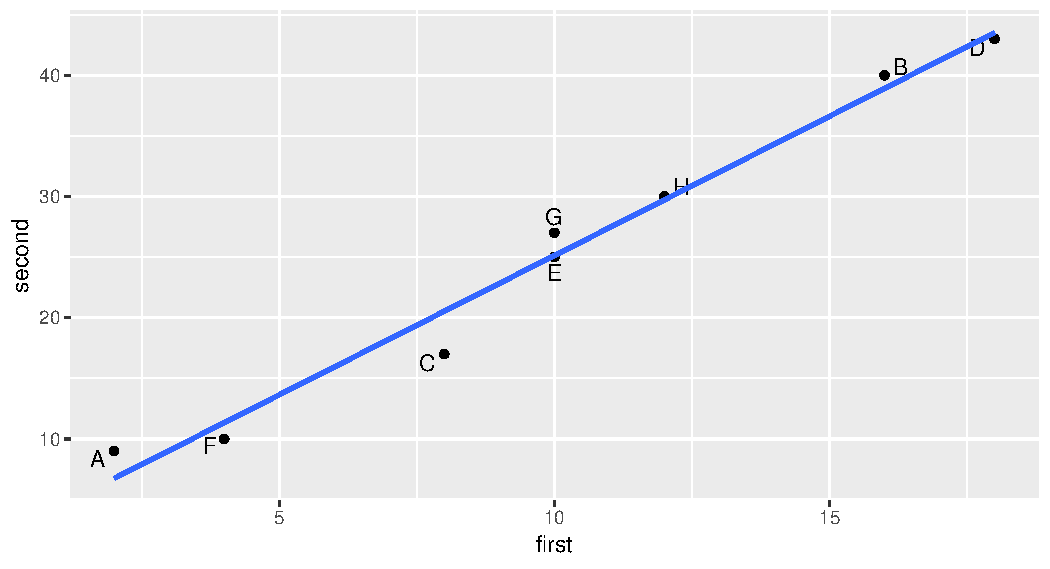
\includegraphics{figure/ff2-1.pdf}
\caption{plot of chunk ff2}
\end{figure}

\end{frame}

\begin{frame}[fragile]{Principal component analysis}
\protect\hypertarget{principal-component-analysis}{}

\begin{itemize}
\tightlist
\item
  Grab just the numeric columns:
\end{itemize}

\begin{Shaded}
\begin{Highlighting}[]
\NormalTok{test12 }\OperatorTok\StringTok{ }\KeywordTok{select_if}\NormalTok{(is.numeric) ->}\StringTok{ }\NormalTok{test12_numbers}
\end{Highlighting}
\end{Shaded}

\begin{itemize}
\tightlist
\item
  Strongly correlated, so data nearly 1-dimensional:
\end{itemize}

\begin{Shaded}
\begin{Highlighting}[]
\KeywordTok{cor}\NormalTok{(test12_numbers)}
\end{Highlighting}
\end{Shaded}

\begin{verbatim}
##           first   second
## first  1.000000 0.989078
## second 0.989078 1.000000
\end{verbatim}

\end{frame}

\begin{frame}[fragile]{Finding principal components}
\protect\hypertarget{finding-principal-components}{}

\begin{itemize}
\tightlist
\item
  Make a score summarizing this one dimension. Like this:
\end{itemize}

\begin{Shaded}
\begin{Highlighting}[]
\NormalTok{test12.pc <-}\StringTok{ }\KeywordTok{princomp}\NormalTok{(test12_numbers, }\DataTypeTok{cor =}\NormalTok{ T)}
\KeywordTok{summary}\NormalTok{(test12.pc)}
\end{Highlighting}
\end{Shaded}

\begin{verbatim}
## Importance of components:
##                          Comp.1      Comp.2
## Standard deviation     1.410347 0.104508582
## Proportion of Variance 0.994539 0.005461022
## Cumulative Proportion  0.994539 1.000000000
\end{verbatim}

\end{frame}

\begin{frame}[fragile]{Comments}
\protect\hypertarget{comments}{}

\begin{itemize}
\item
  ``Standard deviation'' shows relative importance of components (as for
  LDs in discriminant analysis)
\item
  Here, first one explains almost all (99.4\%) of variability.
\item
  That is, look only at first component and ignore second.
\item
  \texttt{cor=T} standardizes all variables first. Usually wanted,
  because variables measured on different scales. (Only omit if
  variables measured on same scale and expect similar variability.)
\end{itemize}

\end{frame}

\begin{frame}[fragile]{Scree plot}
\protect\hypertarget{scree-plot}{}

\begin{Shaded}
\begin{Highlighting}[]
\KeywordTok{ggscreeplot}\NormalTok{(test12.pc)}
\end{Highlighting}
\end{Shaded}

\begin{figure}
\centering
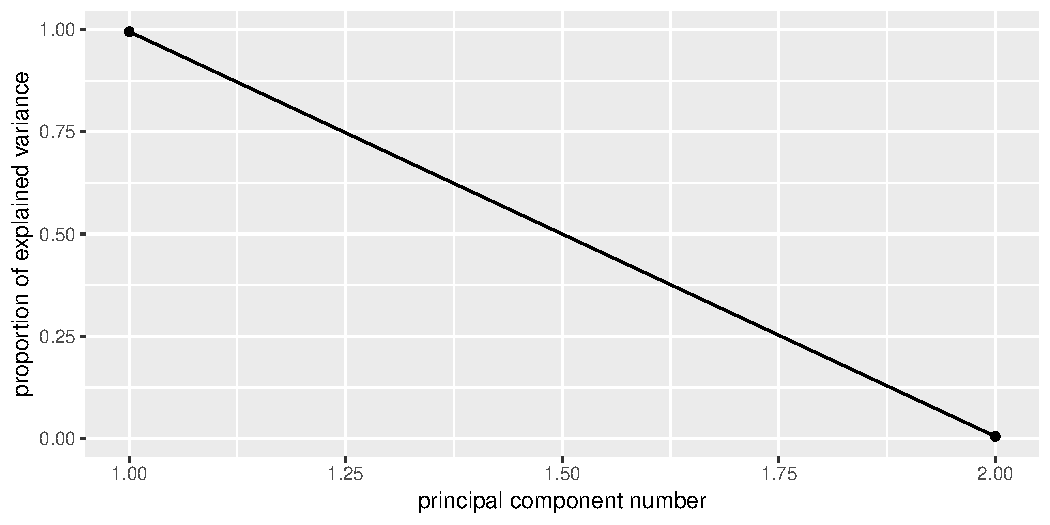
\includegraphics{figure/unnamed-chunk-8-1.pdf}
\caption{plot of chunk unnamed-chunk-8}
\end{figure}

Imagine scree plot continues at zero, so 2 components is a \emph{big}
elbow (take one component).

\end{frame}

\begin{frame}[fragile]{xxx Component loadings}
\protect\hypertarget{xxx-component-loadings}{}

explain how each principal component depends on (standardized) original
variables (test scores):

\footnotesize

\begin{Shaded}
\begin{Highlighting}[]
\NormalTok{test12.pc}\OperatorTok{$}\NormalTok{loadings}
\end{Highlighting}
\end{Shaded}

\begin{verbatim}
## 
## Loadings:
##        Comp.1 Comp.2
## first   0.707  0.707
## second  0.707 -0.707
## 
##                Comp.1 Comp.2
## SS loadings       1.0    1.0
## Proportion Var    0.5    0.5
## Cumulative Var    0.5    1.0
\end{verbatim}

\normalsize

First component basically sum of (standardized) test scores. That is,
person tends to score similarly on two tests, and a composite score
would summarize performance.

\end{frame}

\begin{frame}[fragile]{xxx Component scores}
\protect\hypertarget{xxx-component-scores}{}

\small

\begin{Shaded}
\begin{Highlighting}[]
\NormalTok{d <-}\StringTok{ }\KeywordTok{data.frame}\NormalTok{(test12, test12.pc}\OperatorTok{$}\NormalTok{scores)}
\NormalTok{d}
\end{Highlighting}
\end{Shaded}

\begin{verbatim}
##   first second id       Comp.1       Comp.2
## 1     2      9  A -2.071819003 -0.146981782
## 2    16     40  B  1.719862811 -0.055762223
## 3     8     17  C -0.762289708  0.207589512
## 4    18     43  D  2.176267535  0.042533250
## 5    10     25  E -0.007460609  0.007460609
## 6     4     10  F -1.734784030  0.070683441
## 7    10     27  G  0.111909141 -0.111909141
## 8    12     30  H  0.568313864 -0.013613668
\end{verbatim}

\normalsize

\begin{itemize}
\item
  Person A is a low scorer, high positive \texttt{comp.1} score.
\item
  Person D is high scorer, high negative \texttt{comp.1} score.
\item
  Person E average scorer, near-zero \texttt{comp.1} score.
\item
  \texttt{comp.2} says basically nothing.
\end{itemize}

\end{frame}

\begin{frame}[fragile]{Plot of scores}
\protect\hypertarget{plot-of-scores}{}

\begin{Shaded}
\begin{Highlighting}[]
\KeywordTok{ggplot}\NormalTok{(d, }\KeywordTok{aes}\NormalTok{(}\DataTypeTok{x =}\NormalTok{ Comp}\FloatTok{.1}\NormalTok{, }\DataTypeTok{y =}\NormalTok{ Comp}\FloatTok{.2}\NormalTok{, }\DataTypeTok{label =}\NormalTok{ id)) }\OperatorTok{+}
\StringTok{  }\KeywordTok{geom_point}\NormalTok{() }\OperatorTok{+}\StringTok{ }\KeywordTok{geom_text_repel}\NormalTok{()}
\end{Highlighting}
\end{Shaded}

\begin{figure}
\centering
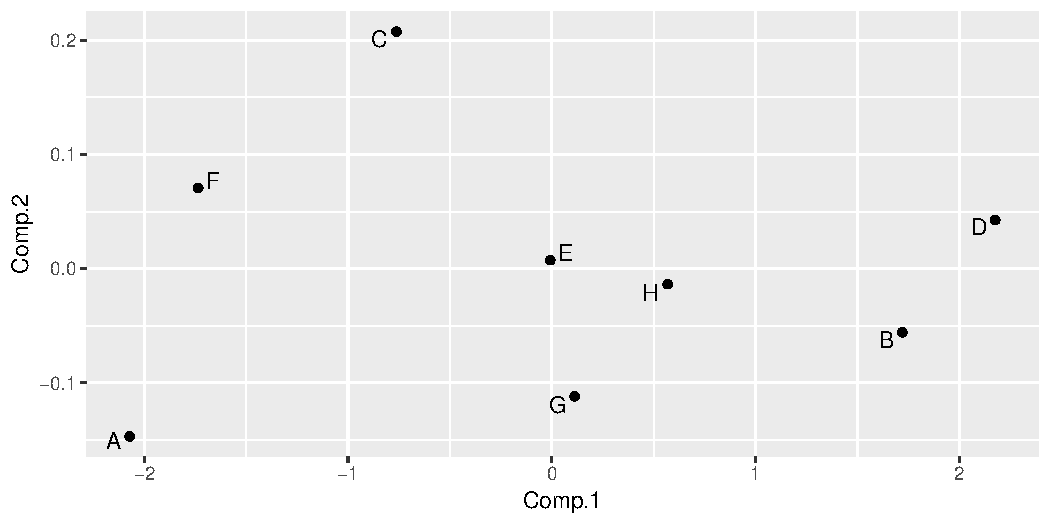
\includegraphics{figure/score-plot-1.pdf}
\caption{plot of chunk score-plot}
\end{figure}

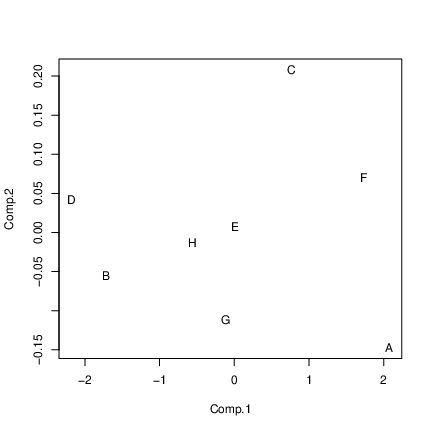
\includegraphics{bPrincomp-score-plot.png}

\end{frame}

\begin{frame}[fragile]{Comments}
\protect\hypertarget{comments-1}{}

\begin{itemize}
\item
  Vertical scale exaggerates importance of \texttt{comp.2}.
\item
  Fix up to get axes on same scale:
\end{itemize}

\begin{Shaded}
\begin{Highlighting}[]
\NormalTok{g <-}\StringTok{ }\KeywordTok{ggplot}\NormalTok{(d, }\KeywordTok{aes}\NormalTok{(}\DataTypeTok{x =}\NormalTok{ Comp}\FloatTok{.1}\NormalTok{, }\DataTypeTok{y =}\NormalTok{ Comp}\FloatTok{.2}\NormalTok{, }\DataTypeTok{label =}\NormalTok{ id)) }\OperatorTok{+}
\StringTok{  }\KeywordTok{geom_point}\NormalTok{() }\OperatorTok{+}\StringTok{ }\KeywordTok{geom_text_repel}\NormalTok{() }\OperatorTok{+}
\StringTok{  }\KeywordTok{coord_fixed}\NormalTok{()}
\end{Highlighting}
\end{Shaded}

\begin{itemize}
\tightlist
\item
  Shows how exam scores really spread out along one dimension:
\end{itemize}

\begin{Shaded}
\begin{Highlighting}[]
\NormalTok{g}
\end{Highlighting}
\end{Shaded}

\begin{figure}
\centering
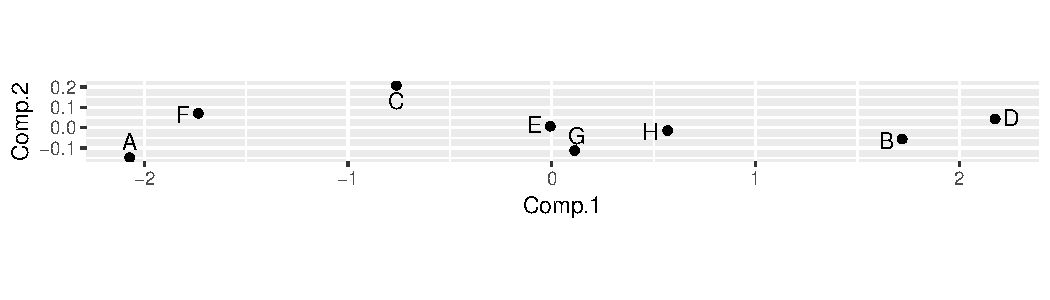
\includegraphics{figure/eqsc2-1.pdf}
\caption{plot of chunk eqsc2}
\end{figure}

\end{frame}

\begin{frame}[fragile]{The biplot}
\protect\hypertarget{the-biplot}{}

\begin{itemize}
\item
  Plotting variables and individuals on one plot.
\item
  Shows how components and original variables related.
\item
  Shows how individuals score on each component, and therefore suggests
  how they score on each variable.
\item
  Add \texttt{labels} option to identify individuals:
\end{itemize}

\begin{Shaded}
\begin{Highlighting}[]
\NormalTok{g <-}\StringTok{ }\KeywordTok{ggbiplot}\NormalTok{(test12.pc, }\DataTypeTok{labels =}\NormalTok{ test12}\OperatorTok{$}\NormalTok{id)}
\end{Highlighting}
\end{Shaded}

\end{frame}

\begin{frame}{The biplot}
\protect\hypertarget{the-biplot-1}{}

\begin{figure}
\centering
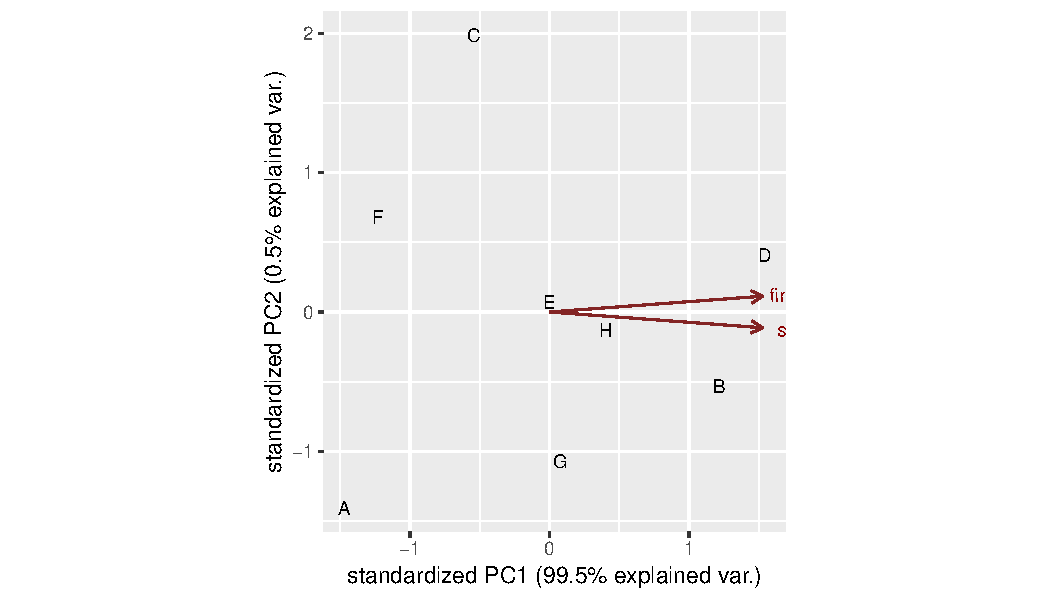
\includegraphics{figure/ff3-1.pdf}
\caption{plot of chunk ff3}
\end{figure}

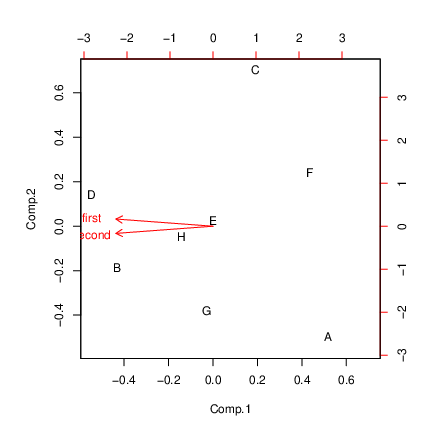
\includegraphics{bPrincomp-test-biplot.png}

\end{frame}

\begin{frame}[fragile]{Comments}
\protect\hypertarget{comments-2}{}

\begin{itemize}
\item
  Variables point almost same direction (left). Thus very negative value
  on \texttt{comp.1} goes with high scores on both tests, and test
  scores highly correlated.
\item
  Position of individuals on plot according to scores on principal
  components, implies values on original variables. Eg.:
\item
  D very negative on \texttt{comp.1}, high scorer on both tests.
\item
  A and F very positive on \texttt{comp.1}, poor scorers on both tests.
\item
  C positive on \texttt{comp.2}, high score on first test relative to
  second.
\item
  A negative on \texttt{comp.2}, high score on second test relative to
  first.
\end{itemize}

\end{frame}

\begin{frame}[fragile]{xxx Track running data}
\protect\hypertarget{xxx-track-running-data}{}

Track running records (1984) for distances 100m to marathon, arranged by
country. Countries labelled by (mostly) Internet domain names (ISO
2-letter codes):

\scriptsize

\begin{Shaded}
\begin{Highlighting}[]
\NormalTok{my_url <-}\StringTok{ "http://www.utsc.utoronto.ca/~butler/d29/men_track_field.txt"}
\NormalTok{track <-}\StringTok{ }\KeywordTok{read_table}\NormalTok{(my_url)}
\NormalTok{track }\OperatorTok\StringTok{ }\KeywordTok{sample_n}\NormalTok{(}\DecValTok{8}\NormalTok{)}
\end{Highlighting}
\end{Shaded}

\begin{verbatim}
## # A tibble: 8 x 9
##    m100  m200  m400  m800 m1500 m5000 m10000 marathon country
##   <dbl> <dbl> <dbl> <dbl> <dbl> <dbl>  <dbl>    <dbl> <chr>  
## 1  10.8  21.9  49    2.02  4.24  16.3   34.7     162. ws     
## 2  10.3  20.7  45.0  1.73  3.6   13.2   27.4     130. be     
## 3  10.4  20.6  45.6  1.76  3.58  13.4   28.2     134. cz     
## 4  10.3  20.8  45.9  1.79  3.64  13.4   27.7     129. jp     
## 5  10.6  21.5  47.8  1.84  3.92  14.7   30.8     149. id     
## 6  10.4  20.8  46.8  1.81  3.7   14.0   29.4     138. ar     
## 7  10.3  20.1  44.8  1.74  3.57  13.3   27.7     128. au     
## 8  10.2  20.6  45.6  1.77  3.61  13.3   27.9     131. se
\end{verbatim}

\normalsize

\end{frame}

\begin{frame}[fragile]{xxx Country names}
\protect\hypertarget{xxx-country-names}{}

Also read in a table to look country names up in later:

\footnotesize

\begin{Shaded}
\begin{Highlighting}[]
\NormalTok{my_url <-}\StringTok{ "http://www.utsc.utoronto.ca/~butler/d29/isocodes.csv"}
\NormalTok{iso <-}\StringTok{ }\KeywordTok{read_csv}\NormalTok{(my_url)}
\NormalTok{iso}
\end{Highlighting}
\end{Shaded}

\begin{verbatim}
## # A tibble: 251 x 4
##    Country        ISO2  ISO3    M49
##    <chr>          <chr> <chr> <dbl>
##  1 <NA>           <NA>  <NA>     NA
##  2 Afghanistan    af    afg       4
##  3 Aland Islands  ax    ala     248
##  4 Albania        al    alb       8
##  5 Algeria        dz    dza      12
##  6 American Samoa as    asm      16
##  7 Andorra        ad    and      20
##  8 Angola         ao    ago      24
##  9 Anguilla       ai    aia     660
## 10 Antarctica     aq    ata      10
## # … with 241 more rows
\end{verbatim}

\normalsize

\end{frame}

\begin{frame}{Data and aims}
\protect\hypertarget{data-and-aims}{}

\begin{itemize}
\item
  Times in seconds 100m--400m, in minutes for rest (800m up).
\item
  This taken care of by standardization.
\item
  8 variables; can we summarize by fewer and gain some insight?
\item
  In particular, if 2 components tell most of story, what do we see in a
  plot?
\end{itemize}

\end{frame}

\begin{frame}[fragile]{xxx Fit and examine principal components}
\protect\hypertarget{xxx-fit-and-examine-principal-components}{}

\footnotesize

\begin{Shaded}
\begin{Highlighting}[]
\NormalTok{track_num <-}\StringTok{ }\NormalTok{track }\OperatorTok\StringTok{ }\KeywordTok{select_if}\NormalTok{(is.numeric)}
\NormalTok{track.pc <-}\StringTok{ }\KeywordTok{princomp}\NormalTok{(track_num, }\DataTypeTok{cor =}\NormalTok{ T)}
\KeywordTok{summary}\NormalTok{(track.pc)}
\end{Highlighting}
\end{Shaded}

\begin{verbatim}
## Importance of components:
##                           Comp.1    Comp.2
## Standard deviation     2.5733531 0.9368128
## Proportion of Variance 0.8277683 0.1097023
## Cumulative Proportion  0.8277683 0.9374706
##                            Comp.3     Comp.4
## Standard deviation     0.39915052 0.35220645
## Proportion of Variance 0.01991514 0.01550617
## Cumulative Proportion  0.95738570 0.97289187
##                             Comp.5      Comp.6
## Standard deviation     0.282630981 0.260701267
## Proportion of Variance 0.009985034 0.008495644
## Cumulative Proportion  0.982876903 0.991372547
##                             Comp.7      Comp.8
## Standard deviation     0.215451919 0.150333291
## Proportion of Variance 0.005802441 0.002825012
## Cumulative Proportion  0.997174988 1.000000000
\end{verbatim}

\normalsize

\end{frame}

\begin{frame}[fragile]{Scree plot}
\protect\hypertarget{scree-plot-1}{}

\begin{Shaded}
\begin{Highlighting}[]
\KeywordTok{ggscreeplot}\NormalTok{(track.pc)}
\end{Highlighting}
\end{Shaded}

\begin{figure}
\centering
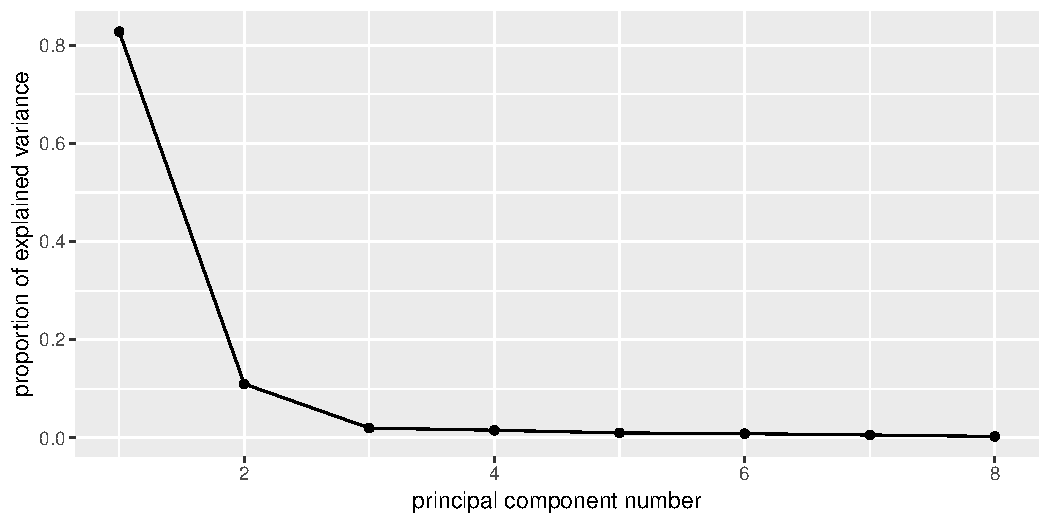
\includegraphics{figure/scree-b-1.pdf}
\caption{plot of chunk scree-b}
\end{figure}

\end{frame}

\begin{frame}[fragile]{How many components?}
\protect\hypertarget{how-many-components}{}

\begin{itemize}
\item
  As for discriminant analysis, look for ``elbow'' in scree plot.
\item
  See one here at 3 components; everything 3 and beyond is ``scree''.
\item
  So take 2 components.
\item
  Note difference from discriminant analysis: want ``large'' rather than
  ``small'', so go 1 step left of elbow.
\item
  Another criterion: any component with eigenvalue bigger than about 1
  is worth including. 2nd one here has eigenvalue just less than 1.
\item
  Refer back to \texttt{summary}: cumulative proportion of variance
  explained for 2 components is 93.7\%, pleasantly high. 2 components
  tell almost whole story.
\end{itemize}

\end{frame}

\begin{frame}[fragile]{xxx How do components depend on original
variables?}
\protect\hypertarget{xxx-how-do-components-depend-on-original-variables}{}

Loadings:

\footnotesize

\begin{Shaded}
\begin{Highlighting}[]
\NormalTok{track.pc}\OperatorTok{$}\NormalTok{loadings}
\end{Highlighting}
\end{Shaded}

\begin{verbatim}
## 
## Loadings:
##          Comp.1 Comp.2 Comp.3 Comp.4 Comp.5 Comp.6 Comp.7 Comp.8
## m100      0.318  0.567  0.332  0.128  0.263  0.594  0.136  0.106
## m200      0.337  0.462  0.361 -0.259 -0.154 -0.656 -0.113       
## m400      0.356  0.248 -0.560  0.652 -0.218 -0.157              
## m800      0.369        -0.532 -0.480  0.540        -0.238       
## m1500     0.373 -0.140 -0.153 -0.405 -0.488  0.158  0.610  0.139
## m5000     0.364 -0.312  0.190        -0.254  0.141 -0.591  0.547
## m10000    0.367 -0.307  0.182        -0.133  0.219 -0.177 -0.797
## marathon  0.342 -0.439  0.263  0.300  0.498 -0.315  0.399  0.158
## 
##                Comp.1 Comp.2 Comp.3 Comp.4 Comp.5 Comp.6 Comp.7
## SS loadings     1.000  1.000  1.000  1.000  1.000  1.000  1.000
## Proportion Var  0.125  0.125  0.125  0.125  0.125  0.125  0.125
## Cumulative Var  0.125  0.250  0.375  0.500  0.625  0.750  0.875
##                Comp.8
## SS loadings     1.000
## Proportion Var  0.125
## Cumulative Var  1.000
\end{verbatim}

\normalsize

\end{frame}

\begin{frame}[fragile]{xxx Comments}
\protect\hypertarget{xxx-comments}{}

\begin{itemize}
\item
  \texttt{comp.1} loads about equally (has equal weight) on times over
  all distances.
\item
  \texttt{comp.2} has large positive loading for short distances, large
  negative for long ones.
\item
  \texttt{comp.3}: large negative for middle distance, large positive
  especially for short distances.
\item
  Country overall good at running will have lower than average record
  times at all distances, so \texttt{comp.1} \emph{small}. Conversely,
  for countries bad at running, \texttt{comp.1} very positive.
\item
  Countries relatively better at sprinting (low times) will be
  \emph{negative} on \texttt{comp.2}; countries relatively better at
  distance running \emph{positive} on \texttt{comp.2}.
\end{itemize}

\end{frame}

\begin{frame}[fragile]{xxx Commands for plots}
\protect\hypertarget{xxx-commands-for-plots}{}

\begin{itemize}
\tightlist
\item
  Principal component scores (first two). Also need country names.
\end{itemize}

\begin{Shaded}
\begin{Highlighting}[]
\NormalTok{d <-}\StringTok{ }\KeywordTok{data.frame}\NormalTok{(track.pc}\OperatorTok{$}\NormalTok{scores,}
  \DataTypeTok{country =}\NormalTok{ track}\OperatorTok{$}\NormalTok{country}
\NormalTok{)}
\KeywordTok{names}\NormalTok{(d)}
\end{Highlighting}
\end{Shaded}

\begin{verbatim}
## [1] "Comp.1"  "Comp.2"  "Comp.3"  "Comp.4"  "Comp.5"  "Comp.6" 
## [7] "Comp.7"  "Comp.8"  "country"
\end{verbatim}

\begin{Shaded}
\begin{Highlighting}[]
\NormalTok{g1 <-}\StringTok{ }\KeywordTok{ggplot}\NormalTok{(d, }\KeywordTok{aes}\NormalTok{(}\DataTypeTok{x =}\NormalTok{ Comp}\FloatTok{.1}\NormalTok{, }\DataTypeTok{y =}\NormalTok{ Comp}\FloatTok{.2}\NormalTok{,}
  \DataTypeTok{label =}\NormalTok{ country)) }\OperatorTok{+}
\StringTok{  }\KeywordTok{geom_point}\NormalTok{() }\OperatorTok{+}\StringTok{ }\KeywordTok{geom_text_repel}\NormalTok{() }\OperatorTok{+}\StringTok{ }\KeywordTok{coord_fixed}\NormalTok{()}
\end{Highlighting}
\end{Shaded}

\begin{itemize}
\tightlist
\item
  Biplot:
\end{itemize}

\begin{Shaded}
\begin{Highlighting}[]
\NormalTok{g2 <-}\StringTok{ }\KeywordTok{ggbiplot}\NormalTok{(track.pc, }\DataTypeTok{labels =}\NormalTok{ track}\OperatorTok{$}\NormalTok{country)}
\end{Highlighting}
\end{Shaded}

\end{frame}

\begin{frame}[fragile]{xxx Principal components plot}
\protect\hypertarget{xxx-principal-components-plot}{}

\begin{Shaded}
\begin{Highlighting}[]
\NormalTok{g1}
\end{Highlighting}
\end{Shaded}

\begin{figure}
\centering
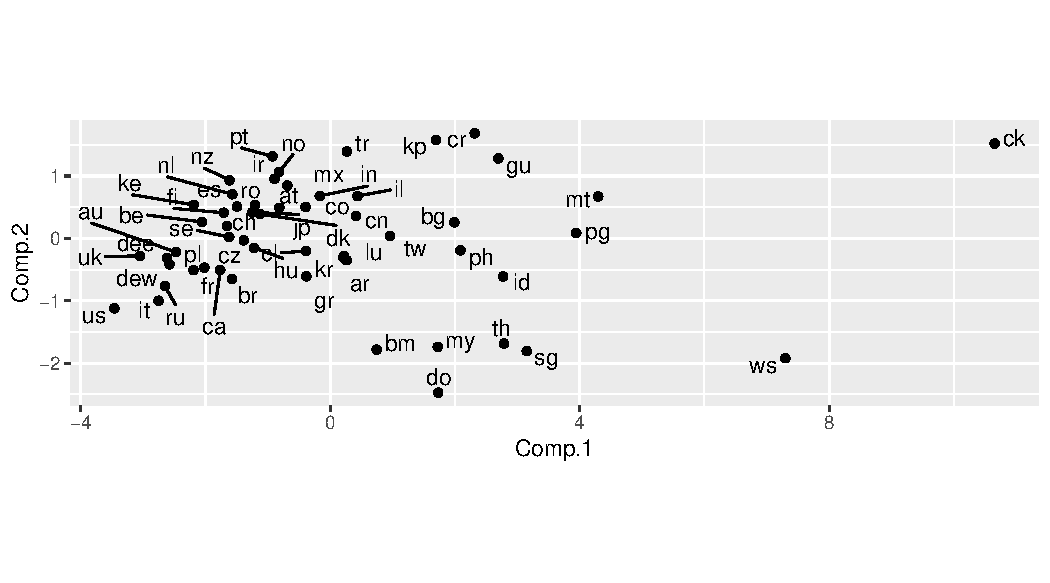
\includegraphics{figure/lecce-1.pdf}
\caption{plot of chunk lecce}
\end{figure}

\end{frame}

\begin{frame}[fragile]{xxx Comments on principal components plot}
\protect\hypertarget{xxx-comments-on-principal-components-plot}{}

\begin{itemize}
\item
  Good running countries at left of plot: US, UK, Italy, Russia, East
  and West Germany.
\item
  Bad running countries at right: Western Samoa, Cook Islands.
\item
  Better sprinting countries at bottom: US, Italy, Russia, Brazil,
  Greece. \texttt{do} is Dominican Republic, where sprinting records
  relatively good, distance records very bad.
\item
  Better distance-running countries at top: Portugal, Norway, Turkey,
  Ireland, New Zealand, Mexico. \texttt{ke} is Kenya.
\end{itemize}

\end{frame}

\begin{frame}[fragile]{xxx Biplot}
\protect\hypertarget{xxx-biplot}{}

\begin{Shaded}
\begin{Highlighting}[]
\NormalTok{g2}
\end{Highlighting}
\end{Shaded}

\begin{figure}
\centering
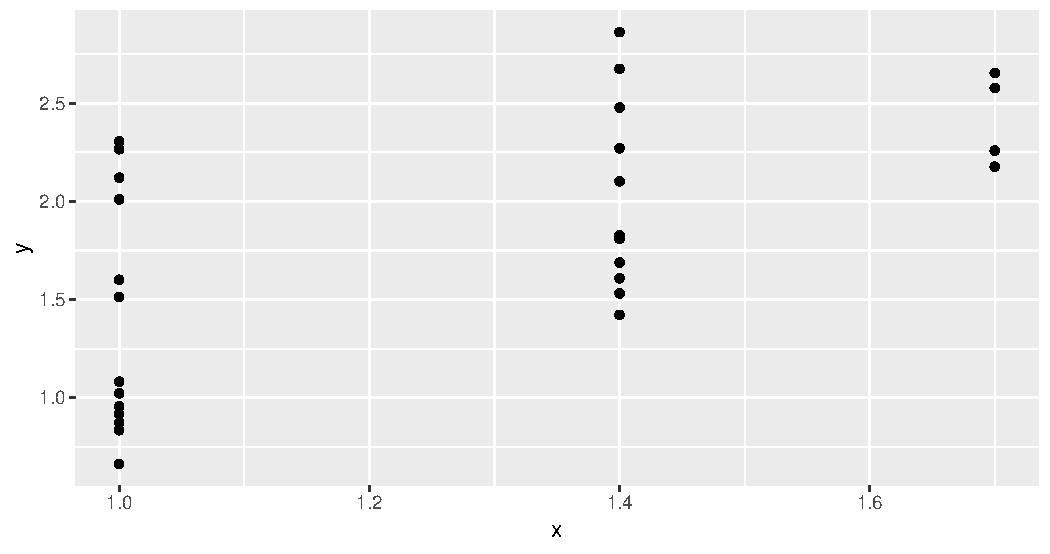
\includegraphics{figure/biplot2-1.pdf}
\caption{plot of chunk biplot2}
\end{figure}

\end{frame}

\begin{frame}{xxx Comments on biplot}
\protect\hypertarget{xxx-comments-on-biplot}{}

\begin{itemize}
\item
  Had to do some pre-work to interpret PC plot. Biplot more
  self-contained.
\item
  All variable arrows point right; countries on right have large (bad)
  record times overall, countries on left good overall.
\item
  Imagine that variable arrows extend negatively as well. Bottom right =
  bad at distance running, top left = good at distance running.
\item
  Top right = bad at sprinting, bottom left = good at sprinting.
\item
  Doesn't require so much pre-interpretation of components.
\end{itemize}

\end{frame}

\begin{frame}[fragile]{xxx Best 8 running countries}
\protect\hypertarget{xxx-best-8-running-countries}{}

Need to look up two-letter abbreviations in ISO table:

xxx \footnotesize

\begin{Shaded}
\begin{Highlighting}[]
\NormalTok{d }\OperatorTok
\StringTok{  }\KeywordTok{arrange}\NormalTok{(Comp}\FloatTok{.1}\NormalTok{) }\OperatorTok
\StringTok{  }\KeywordTok{left_join}\NormalTok{(iso, }\DataTypeTok{by =} \KeywordTok{c}\NormalTok{(}\StringTok{"country"}\NormalTok{ =}\StringTok{ "ISO2"}\NormalTok{)) }\OperatorTok
\StringTok{  }\KeywordTok{select}\NormalTok{(Comp}\FloatTok{.1}\NormalTok{, country, Country) }\OperatorTok
\StringTok{  }\KeywordTok{slice}\NormalTok{(}\DecValTok{1}\OperatorTok{:}\DecValTok{8}\NormalTok{)}
\end{Highlighting}
\end{Shaded}

\begin{verbatim}
##      Comp.1 country                  Country
## 1 -3.462175      us United States of America
## 2 -3.052104      uk           United Kingdom
## 3 -2.752084      it                    Italy
## 4 -2.651062      ru       Russian Federation
## 5 -2.613964     dee             East Germany
## 6 -2.576272     dew             West Germany
## 7 -2.468919      au                Australia
## 8 -2.191917      fr                   France
\end{verbatim}

\normalsize

\end{frame}

\begin{frame}[fragile]{xxx Worst 8 running countries}
\protect\hypertarget{xxx-worst-8-running-countries}{}

\footnotesize

\begin{Shaded}
\begin{Highlighting}[]
\NormalTok{d }\OperatorTok
\StringTok{  }\KeywordTok{arrange}\NormalTok{(}\KeywordTok{desc}\NormalTok{(Comp}\FloatTok{.1}\NormalTok{)) }\OperatorTok
\StringTok{  }\KeywordTok{left_join}\NormalTok{(iso, }\DataTypeTok{by =} \KeywordTok{c}\NormalTok{(}\StringTok{"country"}\NormalTok{ =}\StringTok{ "ISO2"}\NormalTok{)) }\OperatorTok
\StringTok{  }\KeywordTok{select}\NormalTok{(Comp}\FloatTok{.1}\NormalTok{, country, Country) }\OperatorTok
\StringTok{  }\KeywordTok{slice}\NormalTok{(}\DecValTok{1}\OperatorTok{:}\DecValTok{8}\NormalTok{)}
\end{Highlighting}
\end{Shaded}

\begin{verbatim}
##      Comp.1 country          Country
## 1 10.652914      ck     Cook Islands
## 2  7.297865      ws            Samoa
## 3  4.297909      mt            Malta
## 4  3.945224      pg Papua New Guinea
## 5  3.150886      sg        Singapore
## 6  2.787273      th         Thailand
## 7  2.773125      id        Indonesia
## 8  2.697066      gu             Guam
\end{verbatim}

\normalsize

\end{frame}

\begin{frame}[fragile]{xxx Better at distance running}
\protect\hypertarget{xxx-better-at-distance-running}{}

\footnotesize

\begin{Shaded}
\begin{Highlighting}[]
\NormalTok{d }\OperatorTok
\StringTok{  }\KeywordTok{arrange}\NormalTok{(}\KeywordTok{desc}\NormalTok{(Comp}\FloatTok{.2}\NormalTok{)) }\OperatorTok
\StringTok{  }\KeywordTok{left_join}\NormalTok{(iso, }\DataTypeTok{by =} \KeywordTok{c}\NormalTok{(}\StringTok{"country"}\NormalTok{ =}\StringTok{ "ISO2"}\NormalTok{)) }\OperatorTok
\StringTok{  }\KeywordTok{select}\NormalTok{(Comp}\FloatTok{.2}\NormalTok{, country, Country) }\OperatorTok
\StringTok{  }\KeywordTok{slice}\NormalTok{(}\DecValTok{1}\OperatorTok{:}\DecValTok{10}\NormalTok{)}
\end{Highlighting}
\end{Shaded}

\begin{verbatim}
##       Comp.2 country                   Country
## 1  1.6860391      cr                Costa Rica
## 2  1.5791490      kp             Korea (North)
## 3  1.5226742      ck              Cook Islands
## 4  1.3957839      tr                    Turkey
## 5  1.3167578      pt                  Portugal
## 6  1.2829272      gu                      Guam
## 7  1.0663756      no                    Norway
## 8  0.9547437      ir Iran, Islamic Republic of
## 9  0.9318729      nz               New Zealand
## 10 0.8495104      mx                    Mexico
\end{verbatim}

\normalsize

\end{frame}

\begin{frame}[fragile]{xxx Better at sprinting}
\protect\hypertarget{xxx-better-at-sprinting}{}

\footnotesize

\begin{Shaded}
\begin{Highlighting}[]
\NormalTok{d }\OperatorTok
\StringTok{  }\KeywordTok{arrange}\NormalTok{(Comp}\FloatTok{.2}\NormalTok{) }\OperatorTok
\StringTok{  }\KeywordTok{left_join}\NormalTok{(iso, }\DataTypeTok{by =} \KeywordTok{c}\NormalTok{(}\StringTok{"country"}\NormalTok{ =}\StringTok{ "ISO2"}\NormalTok{)) }\OperatorTok
\StringTok{  }\KeywordTok{select}\NormalTok{(Comp}\FloatTok{.2}\NormalTok{, country, Country) }\OperatorTok
\StringTok{  }\KeywordTok{slice}\NormalTok{(}\DecValTok{1}\OperatorTok{:}\DecValTok{10}\NormalTok{)}
\end{Highlighting}
\end{Shaded}

\begin{verbatim}
##        Comp.2 country                  Country
## 1  -2.4715736      do       Dominican Republic
## 2  -1.9196130      ws                    Samoa
## 3  -1.8055052      sg                Singapore
## 4  -1.7832229      bm                  Bermuda
## 5  -1.7386063      my                 Malaysia
## 6  -1.6851772      th                 Thailand
## 7  -1.1204235      us United States of America
## 8  -0.9989821      it                    Italy
## 9  -0.7639385      ru       Russian Federation
## 10 -0.6470634      br                   Brazil
\end{verbatim}

\normalsize

\end{frame}

\begin{frame}[fragile]{Plot with country names}
\protect\hypertarget{plot-with-country-names}{}

\begin{Shaded}
\begin{Highlighting}[]
\NormalTok{g <-}\StringTok{ }\NormalTok{d }\OperatorTok
\StringTok{  }\KeywordTok{left_join}\NormalTok{(iso, }\DataTypeTok{by =} \KeywordTok{c}\NormalTok{(}\StringTok{"country"}\NormalTok{ =}\StringTok{ "ISO2"}\NormalTok{)) }\OperatorTok
\StringTok{  }\KeywordTok{select}\NormalTok{(Comp}\FloatTok{.1}\NormalTok{, Comp}\FloatTok{.2}\NormalTok{, Country) }\OperatorTok
\StringTok{  }\KeywordTok{ggplot}\NormalTok{(}\KeywordTok{aes}\NormalTok{(}\DataTypeTok{x =}\NormalTok{ Comp}\FloatTok{.1}\NormalTok{, }\DataTypeTok{y =}\NormalTok{ Comp}\FloatTok{.2}\NormalTok{, }\DataTypeTok{label =}\NormalTok{ Country)) }\OperatorTok{+}
\StringTok{  }\KeywordTok{geom_point}\NormalTok{() }\OperatorTok{+}\StringTok{ }\KeywordTok{geom_text_repel}\NormalTok{(}\DataTypeTok{size =} \DecValTok{1}\NormalTok{) }\OperatorTok{+}
\StringTok{  }\KeywordTok{coord_fixed}\NormalTok{()}
\end{Highlighting}
\end{Shaded}

\begin{verbatim}
## Warning: Column `country`/`ISO2` joining factor and character
## vector, coercing into character vector
\end{verbatim}

\end{frame}

\begin{frame}[fragile]{The plot}
\protect\hypertarget{the-plot-1}{}

\begin{Shaded}
\begin{Highlighting}[]
\NormalTok{g}
\end{Highlighting}
\end{Shaded}

\begin{figure}
\centering
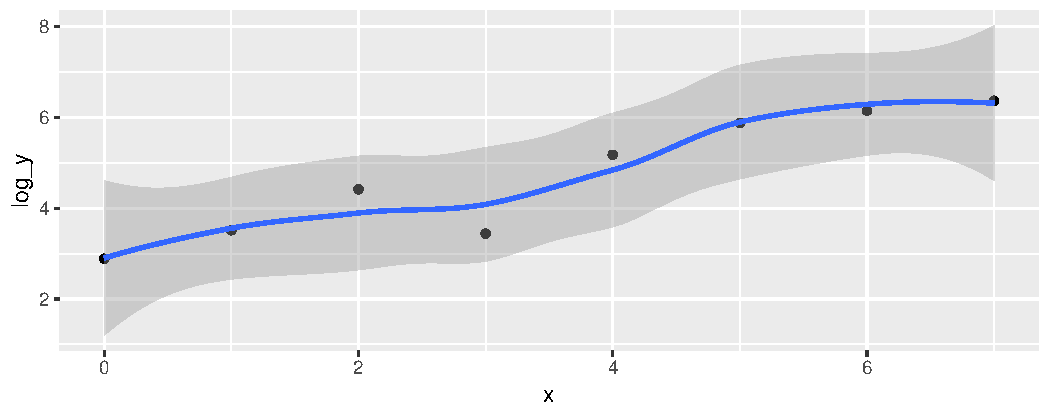
\includegraphics{figure/unnamed-chunk-22-1.pdf}
\caption{plot of chunk unnamed-chunk-22}
\end{figure}

\end{frame}

\begin{frame}[fragile]{xxx Principal components from correlation matrix}
\protect\hypertarget{xxx-principal-components-from-correlation-matrix}{}

Create data file like this:

\begin{verbatim}
 1        0.9705 -0.9600
 0.9705   1      -0.9980
-0.9600  -0.9980  1
\end{verbatim}

and read in like this:

\begin{Shaded}
\begin{Highlighting}[]
\NormalTok{my_url <-}\StringTok{ "http://www.utsc.utoronto.ca/~butler/d29/cov.txt"}
\NormalTok{mat <-}\StringTok{ }\KeywordTok{read_table}\NormalTok{(my_url, }\DataTypeTok{col_names =}\NormalTok{ F)}
\NormalTok{mat}
\end{Highlighting}
\end{Shaded}

\begin{verbatim}
## # A tibble: 3 x 3
##       X1     X2     X3
##    <dbl>  <dbl>  <dbl>
## 1  1      0.970 -0.96 
## 2  0.970  1     -0.998
## 3 -0.96  -0.998  1
\end{verbatim}

\end{frame}

\begin{frame}[fragile]{Pre-processing}
\protect\hypertarget{pre-processing}{}

A little pre-processing required:

\begin{itemize}
\item
  Turn into matrix (from data frame)
\item
  Feed into \texttt{princomp} as \texttt{covmat=}
\end{itemize}

\begin{Shaded}
\begin{Highlighting}[]
\NormalTok{mat.pc <-}\StringTok{ }\NormalTok{mat }\OperatorTok
\StringTok{  }\KeywordTok{as.matrix}\NormalTok{() }\OperatorTok
\StringTok{  }\KeywordTok{princomp}\NormalTok{(}\DataTypeTok{covmat =}\NormalTok{ .)}
\end{Highlighting}
\end{Shaded}

\end{frame}

\begin{frame}[fragile]{Scree plot: one component fine}
\protect\hypertarget{scree-plot-one-component-fine}{}

\begin{Shaded}
\begin{Highlighting}[]
\KeywordTok{ggscreeplot}\NormalTok{(mat.pc)}
\end{Highlighting}
\end{Shaded}

\begin{figure}
\centering
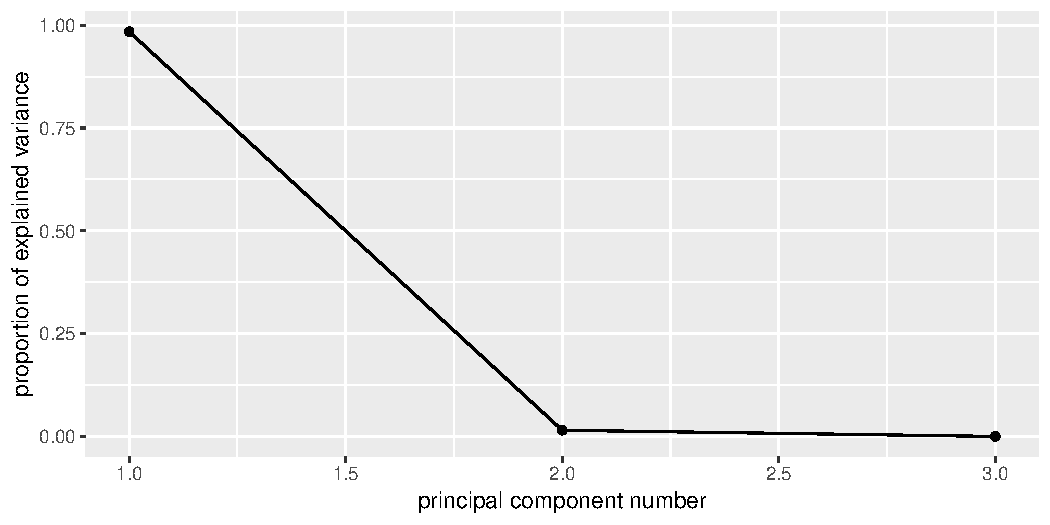
\includegraphics{figure/palermo-1.pdf}
\caption{plot of chunk palermo}
\end{figure}

\end{frame}

\begin{frame}[fragile]{xxx Component loadings}
\protect\hypertarget{xxx-component-loadings-1}{}

Compare correlation matrix:

\scriptsize

\begin{Shaded}
\begin{Highlighting}[]
\NormalTok{mat}
\end{Highlighting}
\end{Shaded}

\begin{verbatim}
## # A tibble: 3 x 3
##       X1     X2     X3
##    <dbl>  <dbl>  <dbl>
## 1  1      0.970 -0.96 
## 2  0.970  1     -0.998
## 3 -0.96  -0.998  1
\end{verbatim}

\normalsize

with component loadings

\scriptsize

\begin{Shaded}
\begin{Highlighting}[]
\NormalTok{mat.pc}\OperatorTok{$}\NormalTok{loadings}
\end{Highlighting}
\end{Shaded}

\begin{verbatim}
## 
## Loadings:
##    Comp.1 Comp.2 Comp.3
## X1  0.573  0.812  0.112
## X2  0.581 -0.306 -0.755
## X3 -0.578  0.498 -0.646
## 
##                Comp.1 Comp.2 Comp.3
## SS loadings     1.000  1.000  1.000
## Proportion Var  0.333  0.333  0.333
## Cumulative Var  0.333  0.667  1.000
\end{verbatim}

\normalsize

\end{frame}

\begin{frame}[fragile]{Comments xxx for sign}
\protect\hypertarget{comments-xxx-for-sign}{}

\begin{itemize}
\item
  When X1 large, X2 also large, X3 small.
\item
  Then \texttt{comp.1} \emph{negative}.
\item
  When X1 small, X2 small, X3 large.
\item
  Then \texttt{comp.1} \emph{positive}.
\end{itemize}

\end{frame}

\begin{frame}{xxx No scores}
\protect\hypertarget{xxx-no-scores}{}

\begin{itemize}
\item
  With correlation matrix rather than data, no component scores
\item
  So no principal component plot
\item
  and no biplot.
\end{itemize}

\end{frame}

\end{document}
